\chapter{Введение} \label{chapt1}
\section{Постановка задачи}
Задачи хранения и обработки большого числа данных встречаются повсеместно. При этом хочется делать это эффективно и быстро. 

Представим себе торговую площадку, каждый товар обладает рядом характеристик непрерывных или дискретных, как например на рисунках~\ref{img:market_example1},~\ref{img:market_example2},~\ref{img:market_example3}.

\begin{figure}[ht] 
	\centering
	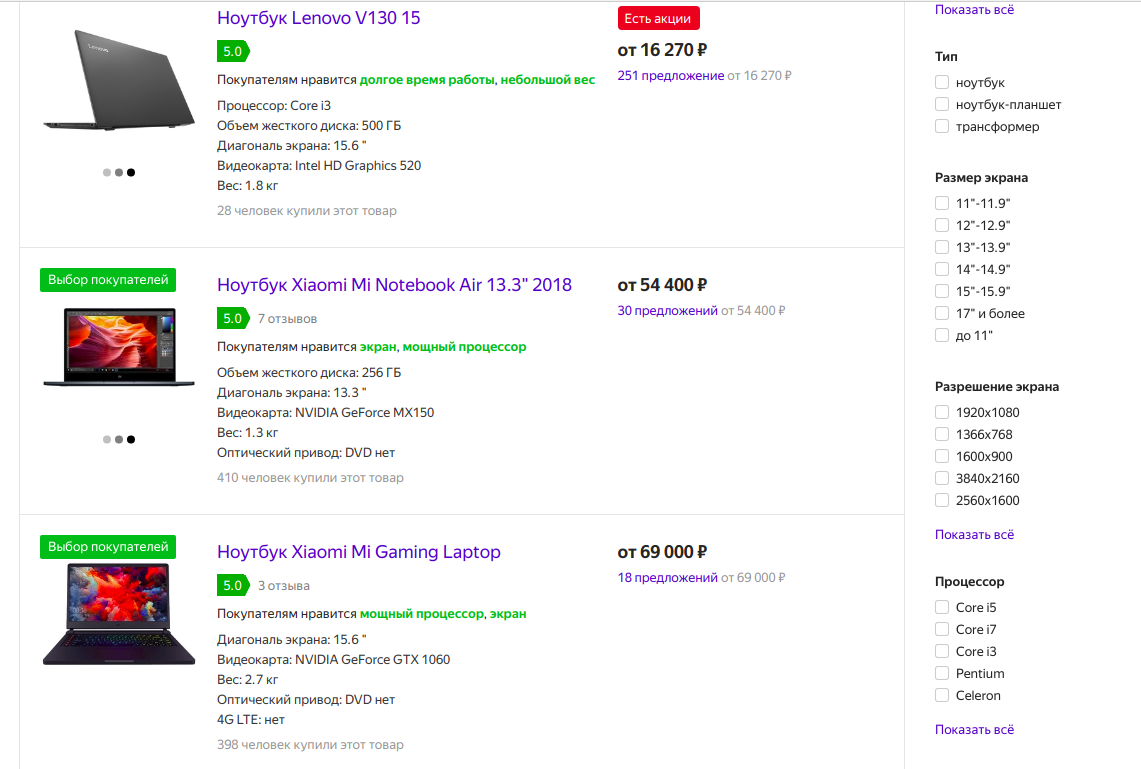
\includegraphics [scale=0.4] {market_example1}
	\caption{Продажа электроники}
	\label{img:market_example1}
\end{figure}

\begin{figure}[ht] 
	\centering
	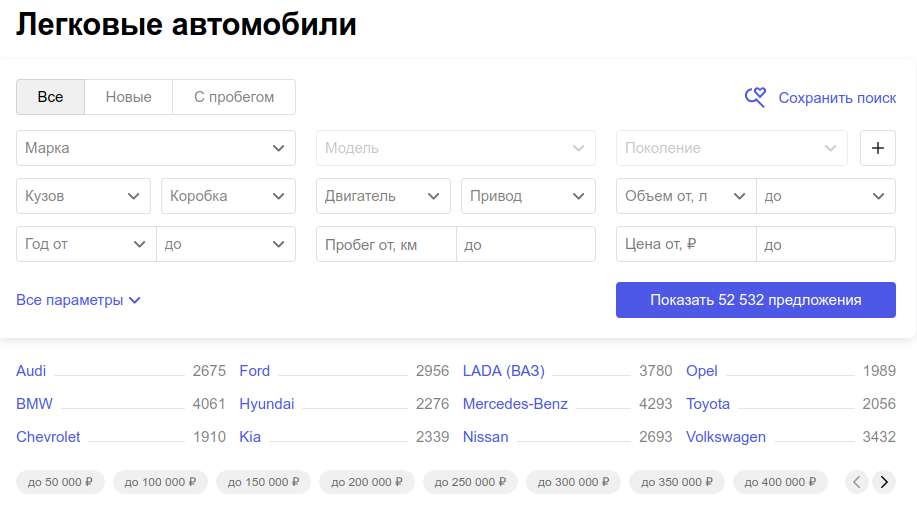
\includegraphics [scale=0.5] {market_example2}
	\caption{Продажа автомобилей}
	\label{img:market_example2}
\end{figure}

\begin{figure}[ht] 
	\centering
	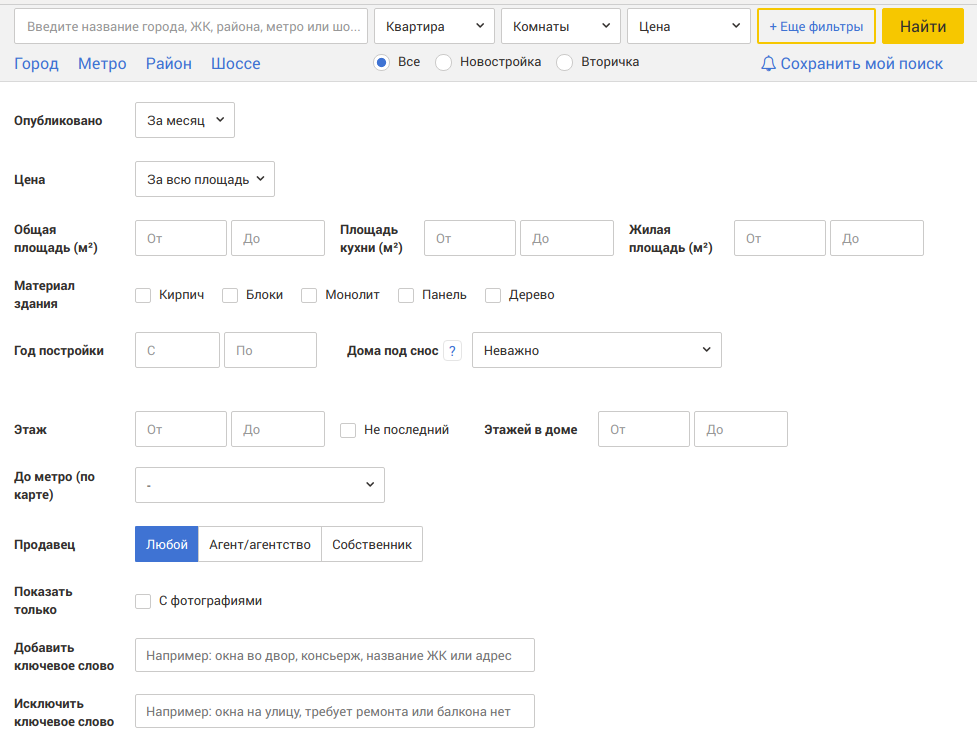
\includegraphics [scale=0.5] {market_example3}
	\caption{Продажа недвижимости}
	\label{img:market_example3}
\end{figure}

Правильно организованная работа с данными увеличивает скорость выполнения запросов и позволяет экономить на оборудовании. Для этого стоит выбрать правильную структуру данных для хранения. Далее будут рассмотрены типы индексов, используемые в современных СУБД и проведено их сравнение. 

\section{Математическая модель}
Сформулируем математическую модель, а также характеристики,
на которых будет сделан акцент в данной работе.

\begin{figure}[ht] 
	\centering
	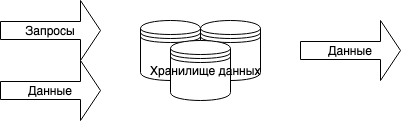
\includegraphics [scale=1] {db_model}
	\caption{Схематическое представление системы хранения данных}
	\label{img:db_model}
\end{figure}

В базовом случае интересующий нас объект --- это хранилище данных~\ref{img:db_model},
обрабатывающее пользовательские запросы. Запросы могут быть
нескольких типов: создание, чтение, обновление и удаление записей.
В зависимости от типа запроса запрашивающая сторона (ей может быть пользователь
или какая-то другая система) должна получить некоторый результат: данные,
удовлетворяющие, условию запроса, если это чтение, и <<подтверждение>> факта, что
данный запрос успешно выполнен.
Важна также корректность результатов наших запросов — если наш запрос
содержит некоторые условия, то при его работе не должны возвращаться,
изменяться и удаляться записи, не удовлетворяющие данному условию. Также
мы не должны иметь побочных эффектов в виде появления записей,
не создаваемых напрямую с помощью запросов или не предусмотренных внутренней
задокументированной логикой работы данной базы данных.

Конечно, обычно СУБД предлагают более широкий список возможностей:
поддержку групп и ролей, разграничение доступа, создание и использование
пользовательских функций, но это не будет рассмотрено, поскольку не имеет
непосредственного отношения к рассматриваемой области.

Не имеет особой разницы форма запроса и ответа на него ---
предполагаем, что существует некоторый протокол, который и используется при общении
с данной СУБД при этом на коммуникацию между системами
тратится сравнимое и меньшее время, чем на выполнение запроса.

Получаемые результаты могут достаточно сильно зависеть от платформы,
на которой будут запускаться тесты.
Более подробное описание среды тестирования, платформы и самих тестов
будет приведено в следующих главах.

\section{Оценка полученных результатов}

Оценка полученных результатов — результат проведения нескольких тестов.
Для начала, считаем, что одна запись — вектор, который содержит числа
и строки. При этом осуществлять поиск планируется не по всем значениям, а
только по их части. Тестирование должно проводится для нескольких размеров
записей: 10/100 байт, 1/10/100 килобайт, 1 мегабайт. Количество полей, по
которым осуществляется поиск стоит взять следующими: 1 (для сравнения со
стандартными решениями), 2, 3 (гео-данные), 5, 20, 50.
На первом этапе стоит проводить вставку 1/10/100 миллионов записей и
замерять количество вставок за единицу времени, а также зависимость этого
времени от количества уже вставленных данных.
Следующий этап – чтение. Для вышеописанных конфигурация измеряется
количество чтений за одну секунду.
Финальный этап наиболее приближен к реальной жизни: должны выполнятся
запросы обоих типов в следующем соотношении — 80/20.
